\documentclass[journal]{IEEEtran}
\usepackage{cite}
\usepackage{amsmath,amssymb,amsfonts}
\usepackage{booktabs}
\usepackage{graphicx}
\usepackage{hyperref}
\usepackage{url}
\usepackage{xcolor}
\usepackage{enumitem}

\title{RAVEN-Select: OCR-Grounded Answer Selection\\for Budgeted Document VQA}

\author{Mohammad Rayaan Raza\\
\normalsize Department of Computer Science\\
\normalsize National University of Computer and Emerging Sciences (FAST-NUCES)\\
\normalsize Islamabad, Pakistan\\
\normalsize Email: 23I-0535@nu.edu.pk}

\begin{document}
\maketitle

\begin{abstract}
High-resolution document visual question answering (Document VQA) is commonly
approximated under limited visual budgets by either resizing the full page or
selecting a few question-relevant patches.  However, better evidence retrieval
does not necessarily yield a better final answer, and no single reader is
uniformly reliable.  We propose \textbf{RAVEN-Select}, a reader-aware,
OCR-grounded answer-output selector.  Three budgeted readers generate answers
from a resized page, BM25-selected patches, and learned-ranker-selected patches.
RAVEN-Select discards empty outputs, identifies generated answers whose
normalized strings occur in page or selected-patch OCR, and returns the shortest
grounded answer; if none is grounded, it falls back to the shortest nonempty
output.  The selector uses no gold-derived feature at inference.  On a
500-question DocVQA validation subset, RAVEN-Select obtains 0.8053 ANLS and
0.706 EM, compared with 0.7840/0.676 for resize and 0.7965/0.688 for the
strongest simple equal-cost heuristic.  Paired bootstrap confidence intervals
for ANLS improvements are $[+0.0062,+0.0380]$ over resize and
$[+0.0023,+0.0173]$ over the shortest-answer heuristic.  Learned output
selectors do not match this statistically supported result at the same scale.
A second-VLM experiment shows the same improvement over the single resize
reader, although the gain over shortest-answer selection is not significant,
indicating that the OCR-grounding advantage is model-dependent.  These results
show that output grounding and selection can be a more important bottleneck
than patch retrieval in budgeted Document VQA.
\end{abstract}

\begin{IEEEkeywords}
Document visual question answering, answer selection, OCR grounding, visual
language models, budgeted inference, model ensembles.
\end{IEEEkeywords}

\section{Introduction}
\IEEEPARstart{D}{ocument} visual question answering requires reading text from
high-resolution, layout-rich images and returning a short answer to a natural
language question.  It builds on text-rich visual question answering, where
models must not only perceive visual content but also read and copy short
textual answers from image text \cite{docvqa,textvqa,m4c}.  Modern visual
language models (VLMs) can process such documents directly, but their
visual-token and memory costs grow with image resolution.  Practical systems
therefore resize an entire page, select a small number of patches, or compress
the visual input \cite{qwen25vl,llavauhd,fastvlm,ureader,docowl2,docvlm}.
This creates a transfer problem: a retrieval method may improve evidence
coverage without improving the answer generated by the downstream reader.

Our experiments expose this gap.  A learned evidence ranker improves patch
coverage, yet its end-to-end answer quality trails a simple resized-page reader.
A retrieve--extract--verify diagnostic achieves high candidate recall but weak
top-1 ranking.  Multiple-choice verification is worse than free generation.
Finally, a learned post-hoc route regressor improves results on 300 examples but
does not significantly beat resize at 500 examples and loses to a simple
shortest-nonempty equal-cost ensemble.  These findings shift the central
question from \emph{which patches should be selected?} to \emph{which generated
answer should be trusted?}

We introduce \textbf{RAVEN-Select} (Reader-Aware, OCR-Grounded Answer
Selection), a deterministic output selector for a small set of budgeted
readers.  The readers observe complementary views: a resized full page,
question-selected lexical patches, and learned-ranker-selected patches.
RAVEN-Select validates each generated output against OCR text already available
from the page or selected patches, then uses answer conciseness to resolve
multiple grounded candidates.  The method is deliberately simple.  Its novelty
lies in treating OCR as an inference-time grounding signal for \emph{generated
answers}, not as a gold-answer diagnostic or as another retrieval target.  The
contribution is not a new VLM architecture; it is a controlled demonstration
that OCR-grounded output selection over complementary budgeted readers can
significantly improve final ANLS and EM.
The central claim is that, under a fixed set of budgeted readers, selecting the
grounded final answer can be more effective than further improving patch
retrieval.

Our contributions are:
\begin{itemize}[leftmargin=*]
  \item We formulate budgeted Document VQA as \emph{answer-output selection}
  among complementary readers rather than as patch selection alone.
  \item We propose a leakage-safe OCR-grounded selector that combines generated
  answer presence and conciseness without using gold answers, oracle routes, or
  gold-derived OCR flags.
  \item We evaluate against single readers, equal-cost heuristics, the previous
  learned route regressor, and four learned selectors using question-level
  out-of-fold evaluation.
  \item On DocVQA $n{=}500$, RAVEN-Select significantly improves ANLS over both
  resize and the strongest simple equal-cost heuristic, while meeting the
  prespecified 0.805 ANLS / 0.705 EM target.
  \item We report exact component, route, cost, and second-VLM ablations,
  including negative results rather than presenting the learned selector as the
  main contribution.
\end{itemize}

\section{Related Work}
\subsection{Document VQA and Document Reading}
DocVQA established question answering over scanned and born-digital document
images \cite{docvqa}.  TextVQA and M4C showed that reading visible text and
copying short OCR tokens are central challenges in visual QA
\cite{textvqa,m4c}.  A separate line of document AI work learns stronger
representations by combining OCR text, layout, and vision, as in LayoutLM and
its successors \cite{layoutlm,layoutlmv2,layoutlmv3,udop}, or removes the
external OCR dependency with image-to-text readers such as Donut and
Pix2Struct \cite{donut,pix2struct}.  RAVEN-Select differs from both: it freezes
the readers and improves the answer-selection interface around their outputs.

\subsection{High-Resolution and Budgeted VLMs}
Text-rich images require more spatial detail than ordinary images.  Recent
systems address this cost through dynamic resolution, slicing, shape-adaptive
cropping, document-token compression, structured OCR/layout encoding, or
efficient visual encoders
\cite{qwen25vl,llavauhd,ureader,docowl2,docvlm,fastvlm}.  RAVEN-Select is
complementary to these architectural approaches.  It neither changes the VLM
nor claims a cheaper encoder; it runs a small fixed set of budgeted readers and
selects their final answer.

\subsection{Budgeted Visual Evidence Selection}
When a full-resolution page exceeds the visual budget, systems may retrieve
text or image regions.  BM25 remains a strong lexical retrieval baseline
\cite{bm25}, while document-image retrieval methods such as ColPali demonstrate
the value of late-interaction visual representations \cite{colpali}.
Retrieval-augmented VQA studies the interaction between evidence retrieval and
generation \cite{ravqa}, and reader-centered passage selection argues that
query relevance and reader usefulness are not identical \cite{readercps}.
Our BM25 and learned evidence routes each expose an overview plus $K=2$
selected patches to the VLM.  Unlike retrieval work, our method does not claim
improved evidence ranking; it selects among answers produced by fixed readers.

\subsection{Answer Reranking and Ensembles}
Answer reranking has been studied in textual QA, including learned candidate
ranking in RankQA \cite{rankqa}.  LLM-Blender uses pairwise ranking and
generative fusion to exploit complementary model outputs \cite{llmblender},
while self-consistency selects an answer supported across multiple generated
reasoning paths \cite{selfconsistency}.  Cost-aware methods such as RouteLLM
and FrugalGPT route queries or build cascades to trade cost against quality
\cite{routellm,frugalgpt}.  RAVEN-Select is closest in spirit to output
selection, but its routing unit is a document-reader answer and its decision
signal is OCR grounding plus conciseness.  We compare learned regression and
LambdaRank selectors (implemented with LightGBM \cite{lightgbm}) against
transparent equal-cost rules.  The central comparison is not against a weak
majority vote but against the strongest observed simple heuristic, shortest
nonempty.

\section{Problem Formulation}
Let $q$ be a question, $I$ a document image, and
\[
\mathcal{R}=\{r_{\mathrm{resize}},r_{\mathrm{BM25}},r_{\mathrm{LER}}\}
\]
the fixed reader set.  Each reader returns a string
$y_r=f_r(I,q)$ under its visual input policy.  The output selector
$s(q,I,\{y_r\})$ chooses one existing answer; it does not synthesize a new
answer.  Let $C_r$ denote reader cost.  The post-generation setting has
$C_{\mathrm{select}}=\sum_{r\in\mathcal{R}}C_r$ plus OCR and negligible string
selection.  Our objective is higher expected ANLS and exact match (EM) than
single readers and selectors with the same three-reader cost.

The setting differs from pre-routing.  A pre-router chooses one reader before
generation and costs one VLM call.  RAVEN-Select is accuracy-oriented and uses
three calls; it is not claimed to be cheaper than resize.

\section{RAVEN-Select}
\subsection{Budgeted Reader Set}
\paragraph{Resize.}
The complete page is resized to the VLM input limit and processed in one call.
It preserves global context but can make small text difficult to read.

\paragraph{BM25 patches.}
OCR text from page regions is scored against the question using BM25
\cite{bm25}.  The VLM receives a page overview and the top $K=2$ patches.

\paragraph{LER-BOPS patches.}
A learned evidence ranker selects $K=2$ patches from the same budgeted pool.
It was developed to improve evidence coverage, but it is retained here as a
complementary reader rather than claimed as the best standalone answerer.

\subsection{Normalization and Grounding}
For a string $y$, the normalization function $N(y)$ lowercases text, removes
punctuation, strips leading and trailing whitespace, and collapses repeated
whitespace.  The same normalization is applied to page OCR $T_{\mathrm{page}}$
and route-specific selected-patch OCR $T_{\mathrm{patch},r}$.

An output is grounded when its nonempty normalized form is a substring of
either OCR source:
\begin{equation}
g_r = \mathbb{1}\!\left[
\begin{aligned}
&N(y_r)\neq\emptyset \ \wedge\\[-2pt]
&\bigl(N(y_r)\subseteq N(T_{\mathrm{page}})\\[-2pt]
&\quad\vee\ N(y_r)\subseteq N(T_{\mathrm{patch},r})\bigr)
\end{aligned}
\right].
\end{equation}
Here $\subseteq$ denotes contiguous string occurrence, not token-set inclusion.
This conservative check supports exact textual answers such as dates, amounts,
names, and short phrases.  It intentionally does not use semantic similarity,
which could introduce another learned component and obscure the source of gain.
Importantly, presence is checked against OCR extracted from the input document,
not against an ``answer OCR'' field or any text derived from the gold answer.
For example, if one reader outputs ``Total Amount Due: 48.50'' and another
outputs ``48.50,'' both may be grounded in the document OCR, but the shorter
grounded output is preferred.

\subsection{Selection Rule}
RAVEN-Select follows answer reranking and multi-output selection rather than
patch selection alone \cite{rankqa,llmblender,selfconsistency}.  Unlike a
learned pairwise ranker or agreement vote, it uses a document-specific
grounding predicate and returns one existing reader output.
Let $\ell_r=|N(y_r)|$ and let $\mathcal{G}=\{r:g_r=1\}$.  RAVEN-Select returns
\begin{equation}
r^\star =
\begin{cases}
\arg\min_{r\in\mathcal{G}} \ell_r, & \mathcal{G}\neq\emptyset,\\
\arg\min_{r:N(y_r)\neq\emptyset} \ell_r, & \text{otherwise}.
\end{cases}
\label{eq:selector}
\end{equation}
Exact length ties are broken deterministically in the order resize, BM25, then
LER-BOPS.  If all outputs are empty, resize is returned.
The first branch rewards answers supported by OCR; the minimum-length rule
penalizes verbose VLM continuations and surrounding sentence text.  The second
branch is the strongest simple equal-cost baseline and supplies a stable
fallback when OCR is incomplete.

\begin{figure}[t]
\centering
\fbox{\begin{minipage}{0.92\columnwidth}
\textbf{Algorithm 1: RAVEN-Select}\\
\textbf{Input:} question $q$, page $I$, outputs
$\{y_{\mathrm{resize}},y_{\mathrm{BM25}},y_{\mathrm{LER}}\}$,
page OCR, selected-patch OCR.\\
1) Normalize all outputs and OCR text.\\
2) Discard empty outputs.\\
3) Mark an output as OCR-grounded if it occurs in page or route-patch OCR.\\
4) If grounded outputs exist, return the shortest grounded output.\\
5) Otherwise, return the shortest nonempty output.\\
6) Break ties by resize, then BM25, then LER-BOPS.
\end{minipage}}
\caption{RAVEN-Select is a deterministic inference-time selector.}
\label{fig:algorithm}
\end{figure}

\subsection{Leakage Safeguards}
The grounding check compares the \emph{generated prediction} with OCR extracted
from the input image or selected patches.  Gold answers are used only after
selection to compute ANLS/EM.  We explicitly exclude:
\begin{itemize}[leftmargin=*]
  \item gold answer text or embeddings;
  \item ANLS or exact match to gold as inference features;
  \item \texttt{answer\_in\_full\_image\_ocr} and
  \texttt{answer\_in\_selected\_patch\_ocr} diagnostic columns, because those
  flags were computed using gold answers;
  \item oracle route identities or any feature derived from ground-truth
  correctness.
\end{itemize}
The OCR-presence cache stores the prediction, OCR text, and prediction-presence
flags per $(\text{question},\text{route},\text{VLM})$.  Model tags are part of
the cache key to prevent robustness-model outputs from sharing flags with the
primary VLM.

\subsection{Learned Selector Comparators}
For completeness, we construct one row per question--route output with
leakage-safe route, prediction-text, question-type, OCR-presence, consensus,
substring, edit-similarity, and retrieval-confidence features.  Training labels
are per-output ANLS to gold, but labels are visible only in training folds.
Five-fold out-of-fold (OOF) evaluation groups rows by question/image so that all
three outputs for a question remain in the same fold.  We compare ridge
regression, logistic best-route classification, LightGBM regression, and
LightGBM LambdaRank.  These are comparators and ablations; none is the primary
method.

\section{Experimental Setup}
\subsection{Data and Models}
We evaluate deterministic subsets of the DocVQA validation split
\cite{docvqa}: a development-scale set of $n=300$ and the primary gate set of
$n=500$.  The principal VLM is Qwen2.5-VL-3B-Instruct in 4-bit mode
\cite{qwen25vl}.  A second-model robustness experiment uses
Qwen2-VL-2B-Instruct on $n=300$.  The primary OCR engine is EasyOCR.  Patch
readers use a page overview and $K=2$ selected patches.

These subsets are not presented as a full-dataset state-of-the-art comparison.
They are controlled, paired experiments over identical questions and cached
reader outputs.

\subsection{Metrics and Statistics}
We report Average Normalized Levenshtein Similarity (ANLS) and exact match (EM).
All comparisons are paired at question level.  Confidence intervals are
percentile bootstrap 95\% intervals over 1,000 resamples with seed 42.  The
prespecified method gate is the $n=500$ result:
\begin{enumerate}[leftmargin=*]
  \item ANLS greater than resize and shortest nonempty;
  \item target ANLS $\geq0.805$ and EM $\geq0.705$;
  \item CI lower bound greater than zero against both resize and shortest
  nonempty.
\end{enumerate}

\subsection{Baselines}
Single-reader baselines are resize, BM25, and LER-BOPS.  Equal-cost
three-reader selectors include normalized majority, resize-on-disagreement,
BM25-on-disagreement, shortest nonempty, answer-type shortest,
consensus-first, and the previous learned RAVEN-post route regressor.  The
strongest simple baseline on $n=500$ is shortest nonempty.
We therefore compare RAVEN-Select only against equal-cost selectors that
consume the same three cached reader outputs, and against one-call readers
separately.

\section{Results}
\subsection{Main Result}
Table~\ref{tab:main500} reports the primary result.  RAVEN-Select improves ANLS
by 0.0214 over resize and by 0.0088 over shortest nonempty.  Both paired
confidence intervals have positive lower bounds.  EM improves by 0.030 over
resize and by 0.018 over shortest nonempty.  The old learned router is below
the simple shortest heuristic at this scale.  The gain is not due to shortest
selection alone: shortest nonempty reaches 0.7965 ANLS, while adding OCR
grounding raises performance to 0.8053.  OCR grounding without the shortest
rule reaches 0.8015, showing that both components matter.

\begin{table}[t]
\centering
\caption{Primary DocVQA result ($n=500$). All selectors below the single-reader
rows consume the same three cached VLM outputs.}
\label{tab:main500}
\begin{tabular}{lcc}
\toprule
Method & ANLS & EM\\
\midrule
Resize (1 call) & 0.7840 & 0.676\\
BM25 (1 call) & 0.7555 & 0.658\\
LER-BOPS (1 call) & 0.7543 & 0.654\\
\midrule
Shortest nonempty & 0.7965 & 0.688\\
OCR-grounded; no shortest & 0.8015 & 0.702\\
Old RAVEN-post & 0.7928 & 0.698\\
Best learned selector & 0.8025 & 0.690\\
\textbf{RAVEN-Select} & \textbf{0.8053} & \textbf{0.706}\\
\bottomrule
\end{tabular}
\end{table}

\begin{figure}[t]
\centering
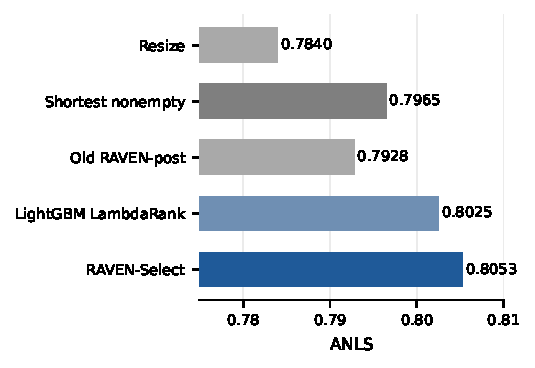
\includegraphics[width=\columnwidth]{figures/fig_main_anls_n500.pdf}
\caption{Primary ANLS comparison on DocVQA $n=500$.  RAVEN-Select's paired
improvement is $+0.0214$ over resize (95\% CI $[+0.0062,+0.0380]$) and
$+0.0088$ over shortest nonempty (95\% CI $[+0.0023,+0.0173]$).}
\label{fig:main-anls}
\end{figure}

\begin{table}[t]
\centering
\caption{Paired ANLS differences for RAVEN-Select on $n=500$.}
\label{tab:ci}
\begin{tabular}{lcc}
\toprule
Comparison & Mean $\Delta$ & 95\% CI\\
\midrule
vs. resize & +0.0214 & $[+0.0062,+0.0380]$\\
vs. shortest nonempty & +0.0088 & $[+0.0023,+0.0173]$\\
\bottomrule
\end{tabular}
\end{table}

\subsection{Development-Scale Result}
On $n=300$, Table~\ref{tab:n300} shows that the same frozen rule obtains 0.8219
ANLS and 0.723 EM.  A learned OOF regressor is higher on this smaller set, but
that ordering reverses on the primary $n=500$ setting.  This instability is why
we do not frame the learned router as the contribution.

\begin{table}[t]
\centering
\caption{DocVQA development-scale results ($n=300$).}
\label{tab:n300}
\begin{tabular}{lcc}
\toprule
Method & ANLS & EM\\
\midrule
Resize & 0.7954 & 0.687\\
Shortest nonempty & 0.8085 & 0.697\\
Old RAVEN-post & 0.8237 & 0.720\\
\textbf{RAVEN-Select} & \textbf{0.8219} & \textbf{0.723}\\
LightGBM OOF (reference) & 0.8324 & 0.733\\
\bottomrule
\end{tabular}
\end{table}

\subsection{Learned Selectors}
Table~\ref{tab:learned} compares the learned output selectors on $n=500$.
LambdaRank is the strongest learned mean at 0.8025, but its CI lower bound is
negative versus shortest nonempty.  The transparent OCR-grounded rule is both
more accurate and statistically supported.  Although learned selectors
approach the rule, their gains over shortest nonempty are not statistically
stable, and they require fold-trained labels.  RAVEN-Select is deterministic,
transparent, and statistically stronger on the primary $n=500$ gate.

\begin{table}[t]
\centering
\caption{Learned OOF selectors on DocVQA $n=500$.}
\label{tab:learned}
\begin{tabular}{lcc}
\toprule
Selector & ANLS & EM\\
\midrule
Logistic best-route & 0.7843 & 0.674\\
Ridge regression & 0.7992 & 0.700\\
LightGBM regression & 0.8005 & 0.698\\
LightGBM LambdaRank & 0.8025 & 0.690\\
\textbf{RAVEN-Select rule} & \textbf{0.8053} & \textbf{0.706}\\
\bottomrule
\end{tabular}
\end{table}

\subsection{Component and Route Ablations}
Table~\ref{tab:ablation} isolates grounding, conciseness, OCR source, and route
contributions.  Removing OCR reduces the method exactly to shortest nonempty
(0.7965).  Removing shortest selection while retaining grounding yields 0.8015,
showing that both components contribute.  Page-only equals the union on this
sample; patch-only has slightly higher ANLS but lower EM, while the frozen
page-or-patch rule gives the strongest balanced endpoint.  Removing either
patch reader lowers performance, with LER removal causing the larger drop.

\begin{table*}[t]
\centering
\caption{Exact RAVEN-Select ablations on DocVQA $n=500$. ``No shortest'' uses
deterministic route priority among grounded outputs.}
\label{tab:ablation}
\begin{tabular}{lccp{7.2cm}}
\toprule
Selector & ANLS & EM & Interpretation\\
\midrule
Resize only & 0.7840 & 0.676 & Best single reader\\
BM25 only & 0.7555 & 0.658 & Lexical patch reader\\
LER-BOPS only & 0.7543 & 0.654 & Learned patch reader\\
Shortest only; no OCR & 0.7965 & 0.688 & Removes grounding\\
OCR-grounded; no shortest & 0.8015 & 0.702 & Removes conciseness\\
Page-OCR + shortest & 0.8053 & 0.706 & Full-page grounding only\\
Patch-OCR + shortest & 0.8065 & 0.698 & Patch grounding only\\
\textbf{Page-or-patch OCR + shortest} & \textbf{0.8053} & \textbf{0.706} & Frozen RAVEN-Select\\
No BM25 route & 0.8023 & 0.700 & Resize + LER only\\
No LER route & 0.7962 & 0.696 & Resize + BM25 only\\
Best learned selector & 0.8025 & 0.690 & LambdaRank, 5-fold OOF\\
\bottomrule
\end{tabular}
\end{table*}

\subsection{Cost and Operating Point}
RAVEN-Select is an accuracy-oriented post-generation selector.  Table
\ref{tab:cost} reports one call per reader and three calls for the method.
The approximate RAVEN-Select runtime is the sum of path medians; it excludes
one-time OCR cache construction and includes negligible cached selection time.
An uncached deployment incurs additional OCR latency.
Accordingly, accuracy comparisons distinguish equal-cost three-output
selectors from one-call reader operating points.

\begin{table}[t]
\centering
\caption{Honest cost accounting on $n=500$.}
\label{tab:cost}
\begin{tabular}{lccc}
\toprule
Method & VLM calls & Median s & ANLS\\
\midrule
Resize & 1 & 2.514 & 0.7840\\
BM25 & 1 & 2.671 & 0.7555\\
LER-BOPS & 1 & 3.519 & 0.7543\\
\textbf{RAVEN-Select} & \textbf{3} & $\mathbf{\sim8.705}$ & \textbf{0.8053}\\
\bottomrule
\end{tabular}
\end{table}

The one-call pre-answer router is retained as a negative result: on $n=500$ it
reaches 0.7762 ANLS versus 0.7840 for resize.  This supports the hypothesis that
post-generation output information is important, but it also means
RAVEN-Select should not be described as a budget-saving pre-router.

\subsection{Second-VLM Robustness}
Table~\ref{tab:qwen2} evaluates the same selector with Qwen2-VL-2B-Instruct on
$n=300$.  RAVEN-Select improves over resize by 0.0291 ANLS with CI
$[+0.0035,+0.0547]$.  It is essentially tied with shortest nonempty: the mean
gain is 0.0002 and the lower confidence bound is zero.  We therefore treat this
as partial robustness: it preserves the improvement over the single resize
reader, while showing that the incremental OCR-grounding advantage over
shortest-answer selection is model-dependent.

\begin{table}[t]
\centering
\caption{Second-VLM robustness ($n=300$, Qwen2-VL-2B).}
\label{tab:qwen2}
\begin{tabular}{lcc}
\toprule
Method & ANLS & EM\\
\midrule
Resize & 0.5980 & 0.537\\
BM25 & 0.4987 & 0.433\\
LER-BOPS & 0.5149 & 0.450\\
Shortest nonempty & 0.6269 & 0.560\\
\textbf{RAVEN-Select} & \textbf{0.6271} & \textbf{0.563}\\
\bottomrule
\end{tabular}
\end{table}

\section{Discussion}
\subsection{Why Grounding and Conciseness Help}
Document answers are frequently short strings copied from the page: names,
dates, totals, percentages, or addresses.  VLM readers can identify the right
region yet produce extra words, explanations, or nearby values.  OCR presence
rejects unsupported generations, while shortest selection removes surrounding
language.  The combination targets final-answer reliability rather than
retrieval coverage.

\subsection{What the Research Arc Reveals}
The sequence of negative and positive findings is informative.  Patch retrieval
alone improved evidence coverage but not final ANLS.  Candidate extraction
reached recall@20 near 0.88 while top-1 ranking remained weak.  Multiple-choice
verification underperformed free generation.  Learned post-hoc routing worked
on $n=300$ but weakened at $n=500$.  The successful intervention acts at the
last transfer step: selecting a grounded final output.  Thus, in this budgeted
setting, answer grounding matters more than another patch-retrieval refinement.
Our raw OCR-text augmentation was also not the winning interface.  This is
consistent with work arguing that structured OCR/layout compression can be more
effective than simply appending raw OCR strings to a VLM \cite{docvlm}.

\subsection{Simplicity Versus Learned Routing}
RAVEN-Select has no learned parameters.  This is a strength only because the
comparison is fair: all three-reader selectors consume the same cached outputs,
and the simple method beats learned regressors and the strongest heuristic with
paired statistical support.  The result should not be interpreted as evidence
that learned selection is generally unnecessary; rather, the available
$n=500$ data and feature set do not justify its additional complexity.

\section{Limitations}
\begin{itemize}[leftmargin=*]
  \item \textbf{Three VLM calls.}  RAVEN-Select improves accuracy but is more
  expensive than a one-call resize reader.  It is an equal-cost multi-reader
  selector, not a cheap pre-router.
  \item \textbf{Subset scale and one main dataset.}  The statistically supported
  result is on a 500-question DocVQA validation subset, not the full benchmark
  or a second document dataset.  Multi-page and table-heavy settings may
  require page localization and explicit row/cell reasoning beyond output
  selection \cite{mpdocvqa,tapas,docowl2}.
  \item \textbf{Second-model uncertainty.}  Qwen2-VL-2B retains the gain over
  resize but not a positive CI lower bound over shortest nonempty.
  \item \textbf{OCR dependence.}  Exact substring grounding can reject correct
  paraphrases and inherit OCR errors.  Earlier retrieval experiments also show
  sensitivity when changing OCR engines.
  \item \textbf{Best-of-reader ceiling.}  Because RAVEN-Select chooses among
  generated outputs, it cannot recover an answer that none of the readers
  generate.  Its ceiling is therefore bounded by the best-of-reader oracle,
  which reaches 0.8333 ANLS on the primary subset versus 0.8053 for the method.
  \item \textbf{Language and answer form.}  The method is best suited to
  extractive short answers.  Long-form, abstractive, multilingual, or heavily
  normalized answers may not occur verbatim in OCR.
  \item \textbf{Patch-only ANLS.}  Patch-only grounding is 0.0012 higher in
  mean ANLS on $n=500$ but 0.008 lower in EM than the frozen union rule.
  Broader evaluation is needed to determine whether this trade-off generalizes.
\end{itemize}

\section{Conclusion}
We presented RAVEN-Select, a simple OCR-grounded answer-output selector for
budgeted Document VQA.  Instead of further optimizing patch retrieval, the
method runs three complementary readers and selects the shortest nonempty
generated answer supported by page or patch OCR.  On DocVQA $n=500$, it
improves ANLS from 0.7840 to 0.8053 over resize and from 0.7965 to 0.8053 over
the strongest simple equal-cost selector, with paired confidence intervals
above zero.  The result supports a broader conclusion: when better evidence
does not transfer to better answers, grounding and output selection can be the
more consequential design problem.

\section*{Reproducibility}
All selectors operate on cached per-question outputs.  The main commands are:
\begin{verbatim}
python scripts/run_raven_select_build_features.py --n 500
python scripts/run_raven_select_eval.py --n 500 --write-gates
python scripts/run_raven_select_paper_ablations.py --n 500
\end{verbatim}
Primary artifacts are
\texttt{raven\_select\_overview\_n500.json},
\texttt{raven\_select\_paper\_ablations\_n500.csv}, and gate reports P14--P16.

\bibliographystyle{IEEEtran}
\bibliography{references}

\end{document}
